
\subsubsection{08.11.14}

\begin{enumerate}
	\item The time of beginning and ending of the meeting:
	16:00 - 20:00
	\item Purposes of the meeting:
	\begin{enumerate}
		\item To elaborate new ideas for MCB.
		
		\item To start creating MCB.
		
	\end{enumerate}
	
	\item Work that has been done:
	\begin{enumerate}
		\item Ideas of the capture mechanism's construction:
		\begin{enumerate}
			\item Mechanism that consist of two vertical rails that can turn. Then beams move apart in hand and pumps on the base of basket. Pluses: compact and easy assembly. Minus of this construction is that it can capture only one basket (it is not profitable in the autonomous period and in the final). Also it will need to aim for capture basket.
			
			\item The mechanism that consists two beams that can fall on both sides of the movable baskets. Then the basket base compress between the two beams. Pluses: beams may additionally lengthen so robot will be able to capture two baskets. This mechanism is simpler because it does not need to aim carefully. Minuses: uncompact, heaviness.
		
			\begin{figure}[H]
				\begin{minipage}[h]{0.2\linewidth}
					\center  
				\end{minipage}
				\begin{minipage}[h]{0.6\linewidth}
					\center{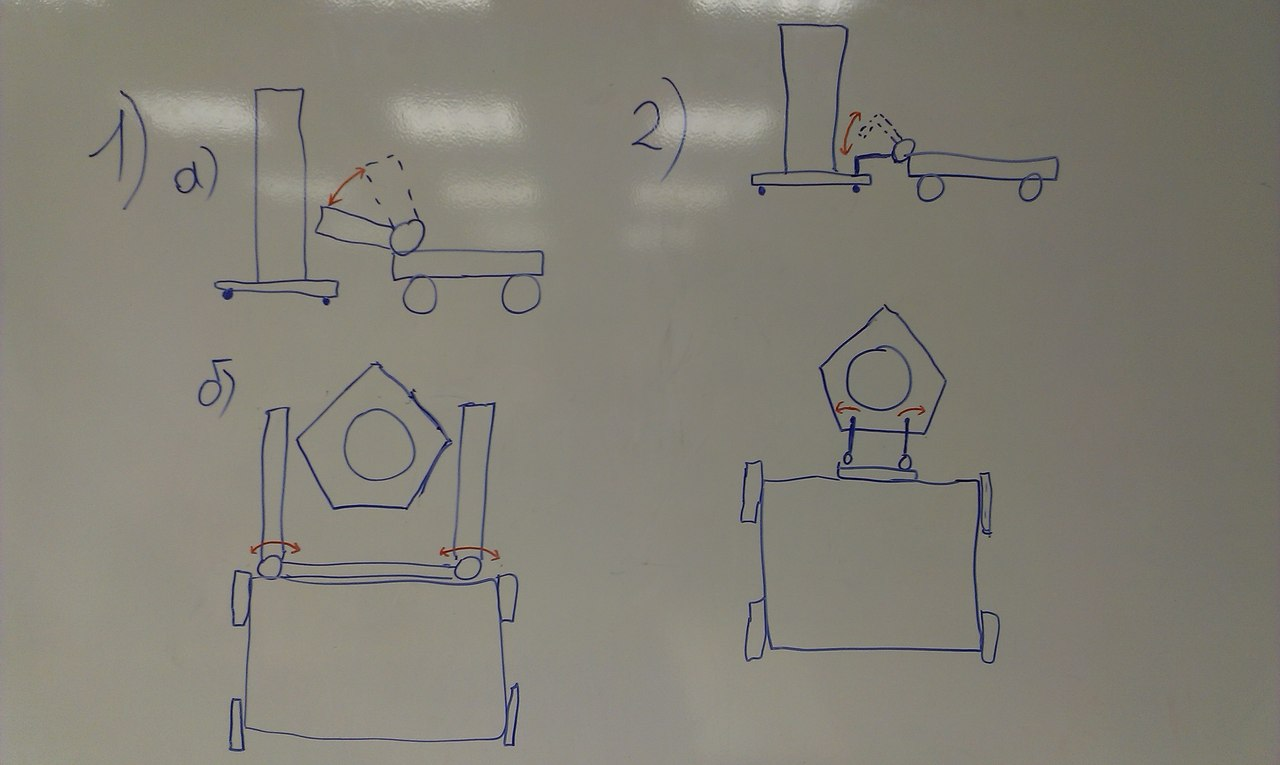
\includegraphics[scale=0.2]{days/08.11.14/images/01}}
					\caption{Ideas of capture of movable baskets: 1)Two beams 2)Vertical slats %-1 3)Клешни-2
						}
				\end{minipage}
			\end{figure}
			
		\end{enumerate}
		
		\item Asembly of MCB is not started because we didn't choose it.
		
		\item It was decided to use the hole for servo for power button.
		
		\begin{figure}[H]
			\begin{minipage}[h]{0.2\linewidth}
				\center  
			\end{minipage}
			\begin{minipage}[h]{0.6\linewidth}
				\center{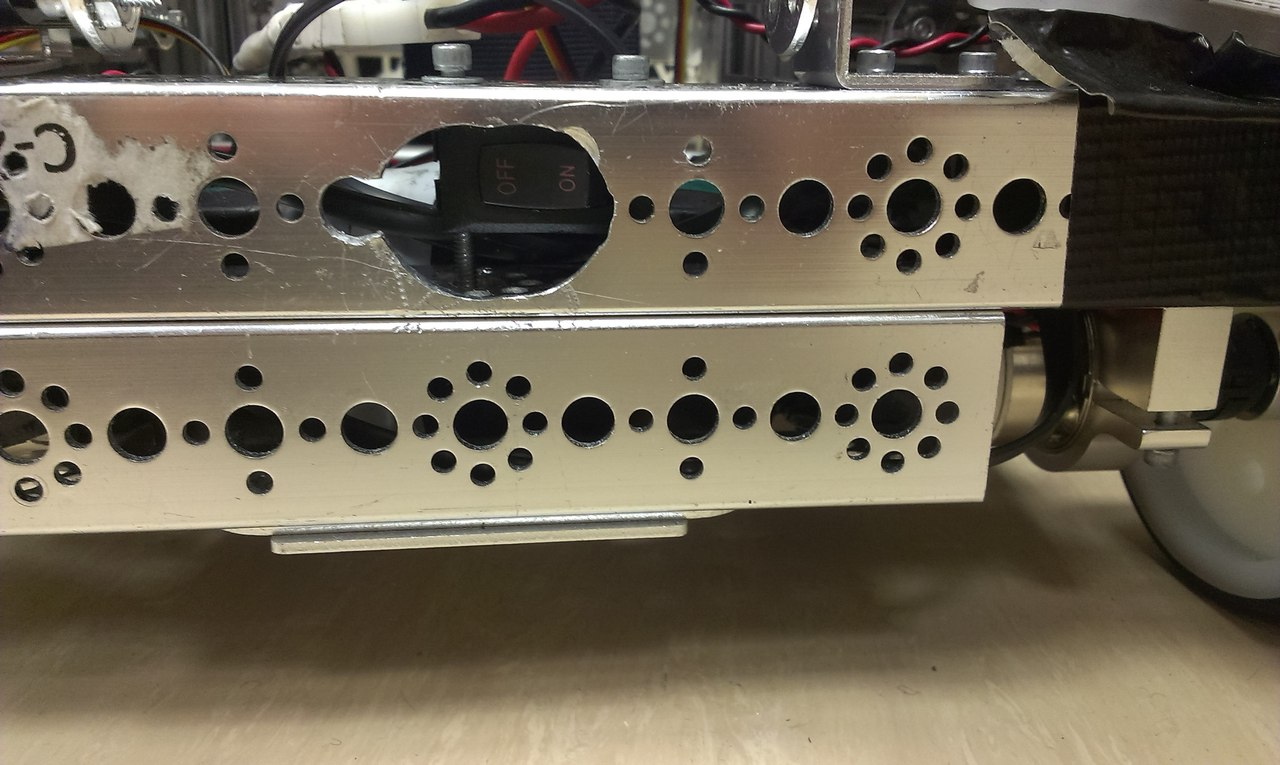
\includegraphics[scale=0.2]{days/08.11.14/images/02}}
				\caption{Button of power}
			\end{minipage}
		\end{figure}
		
	\end{enumerate}
	
	\item Results:  
	\begin{enumerate}
		\item Three ideas of design have been suggested.
		
		\item The MCB is not implemented.
		
	\end{enumerate}
	
	\item Tasks for the next meetings:
	\begin{enumerate}
		\item To choose the optimal variant of MCB.
		
		\item To assemble MCB.
		
	\end{enumerate}     
\end{enumerate}
\fillpage

